% ============================================================================
% AAAI-27 anonymous submission draft.
% Evidence freeze: 2026-07-16.
% Compile: pdflatex -> bibtex -> pdflatex -> pdflatex.
% ============================================================================
\documentclass[letterpaper]{article}
\usepackage[submission]{aaai2027}
\usepackage[hyphens]{url}
\usepackage{graphicx}
\urlstyle{rm}
\def\UrlFont{\rm}
\usepackage{natbib}
\usepackage{caption}
\frenchspacing
\usepackage{booktabs}
\usepackage{amsmath}
\usepackage{array}
\pdfinfo{
/TemplateVersion (2027.1)
}

\setcounter{secnumdepth}{2}

\title{When Shared Experience Becomes an Implementation Attractor: Lock-In, Mitigation, and Task Boundaries in Parallel LLM Agents}
\author{Anonymous Submission}
\affiliations{}

\begin{document}
\maketitle

\begin{abstract}
Parallel LLM agents are often made more capable by broadcasting prior outputs or
manager-synthesized experience to later agents. We audit a risk that is weaker than
catastrophic failure but easier to miss: shared experience may suppress independent
solutions and stabilize a common implementation attractor. We instantiate a layered
Mixture-of-Agents coding system with three private MiniSWE workspaces per layer,
blinded experience transfer, and hidden executable evaluation. In a frozen
12-layer, three-arm Kimi-K2.6 experiment on a 37-test SlopCodeBench task, cumulative
self-reported experience does not reproduce the preregistered sustained
degradation curve. Instead, all workers share the same failed-test signature from
layer 3 and the same exact implementation from layer 5, remaining at 33/37 through
layer 12. Retrospective audits of two independent cumulative trajectories
reproduce consecutive exact-snapshot lock-in from layers 3 and 4. A prospectively
frozen fixed-three-reference control produces one primary implementation from
layers 2--6, showing that cumulative history growth is unnecessary. A local-only
diversity router increases post-layer-1 diversity AUC from 5 to 6 and delays
lock-in from layer 2 to layer 3 without changing 34/37 quality, but does not
prevent it. On a prospectively frozen same-provider \texttt{log\_query} boundary,
all arms retain three implementations through layer 3, while transfer improves
mean all-test count from 108.4/134 to 127.2/134 and 130.1/134. Experience
therefore creates a conditional quality--diversity trade-off rather than a
universal multi-agent ``death spiral.'' A local completion-and-smoke gate
additionally blocks two zero-command false completions, but rejects five strong
solutions at its frozen threshold.
\end{abstract}

\section{Introduction}

Army ants can form a circular mill when locally sensible trail-following becomes
self-reinforcing at the colony level~\citep{schneirla1944circularmill}. The analogy
is tempting for multi-agent LLM systems: each imported lesson can be plausible,
each recipient can appear successful, and yet repeated sharing can remove the
independence that made parallel agents useful. The analogy, however, is not
evidence. This paper asks a narrower, executable question: \emph{what actually
happens when parallel coding agents repeatedly absorb shared experience?}

Layered Mixture-of-Agents (MoA) systems let several agents solve the same task and
then expose later agents to earlier outputs~\citep{wang2024moa}. Experience-driven
agents similarly distill trajectories into reusable textual guidance
\citep{zhao2024expel,shinn2023reflexion}, and multi-agent development systems share
messages, roles, or cross-task experience
\citep{qian2024chatdev,qian2024colearning,li2025mael_full}. These mechanisms can
improve accuracy and efficiency. They can also correlate recipients: once a
privileged shared artifact is accepted, later ``independent'' workers may inherit
the same assumptions, tests, and omissions.

Recent work has identified semantic anchoring and diversity collapse in
multi-agent discussion~\citep{guo2026diversitycollapse,zhang2026semanticcollapse}.
Our focus is complementary. We study \emph{experience-mediated lock-in} in an
executable workflow where each agent edits a private repository, external tests
measure exact behavior, and implementation identity can be audited by snapshot
hash. This setting separates three outcomes that are often conflated:
(i) performance collapse, (ii) implementation lock-in, and (iii) behavioral
lock-in despite distinct code.

We initially sought a sustained degradation curve: as accepted experience
accumulates, correct but increasingly complex guidance might trigger false
completion and then propagate it. The strongest frozen replication rejects that
story. The more reproducible finding is subtler. Cumulative experience rapidly
homogenizes behavior and sometimes exact code, while catastrophic outcomes remain
stochastic, model-dependent, and recoverable. A local admission rule blocks the
observed zero-command false completions, but its threshold also discards strong
solutions. Independent trajectory audits reproduce exact implementation lock-in,
and a fixed-three-reference control shows that it can occur without a growing
history. Recursive synthesis can lock agents onto an inferior fixed point on one
task and improve them on another. A local-only diversity router delays rather
than prevents lock-in on \texttt{cfgpipe}, while a same-provider
\texttt{log\_query} probe preserves maximal implementation diversity and improves
quality under transfer.

Our contributions are:
\begin{itemize}
    \item an audited layered MoA coding testbed with private workspaces, barrier
    synchronization, blinded transfer, hidden external evaluation, and an exact
    experience-artifact specification;
    \item a preregistered negative result showing that depth and context growth do
    not reproducibly yield a sustained degradation curve across three model
    families;
    \item replicated trajectory and source-alignment evidence of an implementation
    attractor, plus a prospective fixed-reference control showing that cumulative
    history growth is not required in the tested setting;
    \item a prospective local-diversity router that yields only a one-layer delay,
    together with a same-provider second-task boundary where transfer improves
    quality without reducing implementation diversity; and
    \item a trajectory-level admission audit that quantifies the trade-off between
    rejecting false completion and retaining high-quality experience.
\end{itemize}

\section{Related Work}

\paragraph{Experiential agents and shared memory.}
ExpeL distills reusable insights from agent trajectories
\citep{zhao2024expel}; Reflexion stores verbal feedback for subsequent attempts
\citep{shinn2023reflexion}; Generative Agents and MemoryBank manage longer-term
retrieval and salience~\citep{park2023generative,zhong2024memorybank}. Experiential
co-learning extends this idea to software-development teams
\citep{qian2024colearning}, while MAEL maintains cross-task experience in a
collaboration graph~\citep{li2025mael_full}. These works motivate transfer as a
capability mechanism. We audit what happens when accepted experience becomes a
shared, recursively reused coordination state.

\paragraph{Parallel and role-based multi-agent systems.}
MoA uses layered parallel proposers and an aggregator
\citep{wang2024moa}. ChatDev and MetaGPT coordinate specialized software roles
\citep{qian2024chatdev,hong2024metagpt}; AgentVerse and MultiAgentBench study
collaborative and competitive interaction
\citep{chen2023agentverse,zhu2025multiagentbench}. Multi-agent debate aggregates
reasoning rather than persistent experience~\citep{du2024debate}. Our workers
instead solve the same coding task in private workspaces, so diversity is
operational: agents may produce different repository states that pass and fail
different tests.

\paragraph{Conformity and executable coding evaluation.}
Semantic anchoring can manufacture agreement and reduce diversity in LLM
collectives~\citep{guo2026diversitycollapse,zhang2026semanticcollapse}. We connect
that concern to executable consequences by measuring exact snapshot hashes and
failed-test sets. SlopCodeBench evaluates coding agents against iteratively
revealed specifications and hidden executable tests
\citep{orlanski2026slopcode}. Its checkpointed projects provide a controlled
middle ground between toy reasoning tasks and unconstrained repository issues such
as SWE-bench~\citep{jimenez2024swebench}.

\section{Audited Parallel-Agent Testbed}
\label{sec:method}

\subsection{Topology and Isolation}

Figure~\ref{fig:system} shows the fixed topology. At each layer, three MiniSWE
workers receive the same public task and run concurrently in private repository
workspaces. A barrier closes the layer before any output is shared. The next layer
receives a policy-selected experience state; no worker sees another worker's live
workspace. An external evaluator then runs the frozen tests on each snapshot.
External pass counts, failed-test names, and collection hashes are withheld from
workers and from self-report or local-admission recipients.

\begin{figure*}[t]
\centering
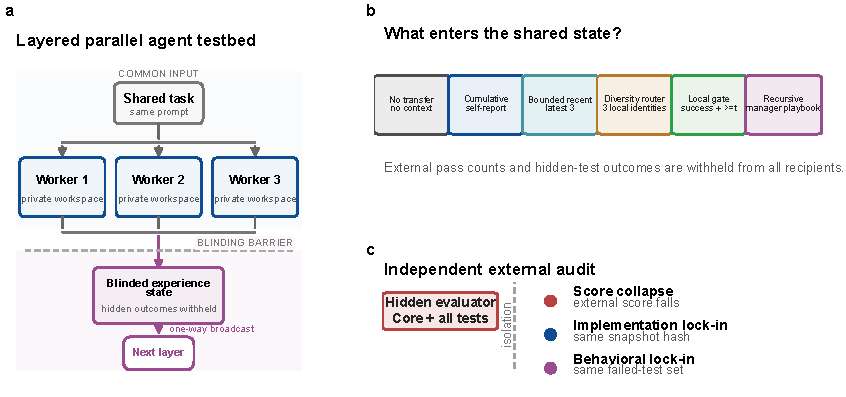
\includegraphics[width=\textwidth]{figures/moa/figure1_moa_system.pdf}
\caption{\textbf{Audited layered parallel-agent testbed.}
\textbf{a}, Three MiniSWE workers solve the same task concurrently in private
workspaces; a barrier closes the layer before a blinded experience state is
broadcast. \textbf{b}, Policies differ only in what enters that state: nothing,
self-reported success, a fixed recent window, a local implementation-diversity
router, self-report plus a local command threshold, or one recursively synthesized
manager playbook.
\textbf{c}, A hidden evaluator separately
measures external score, implementation identity, and failed-test behavior.
External outcomes are never delivered to self-report or local-admission
recipients.}
\label{fig:system}
\end{figure*}

The implementation uses AutoGen Core's routed-agent runtime for the barrier and
message topology, and the pinned native MiniSWE runner from SlopCodeBench for
agent--environment interaction. We remove reference solutions, later checkpoint
specifications, and hidden evaluator paths from worker-visible workspaces. Every
interpreted result must match the frozen test count and collection hash, contain a
valid model query, and pass a prohibited-access scan.

\subsection{Transfer Policies}

Table~\ref{tab:policies} defines the policies. \textbf{No transfer} suppresses all
prior outputs. \textbf{Cumulative self-report} admits every output whose trajectory
claims successful completion and appends its bounded experience summary to the
shared history. \textbf{Bounded recent transfer} uses the same admission signal
but retains only the three most recent accepted outputs. \textbf{Bounded diverse
transfer} retains the latest three locally distinct implementation identities
across bootstrap and completed layers. \textbf{Local admission} additionally
requires at least three
successful environment commands; this is an agent-local completion-and-smoke
proxy, not external verification. \textbf{Recursive synthesis} sends accepted
outputs and the previous shared playbook to a manager, which emits one revised
playbook for the next layer.

\begin{table}[t]
\centering
\caption{Transfer and admission policies. ``Hidden'' means external evaluator
outcomes are withheld from recipients.}
\label{tab:policies}
\begin{tabular}{p{0.20\columnwidth}p{0.32\columnwidth}p{0.25\columnwidth}}
\toprule
Policy & Shared state & Admission signal \\
\midrule
No transfer & Empty & None \\
Self-report & All accepted summaries to date & Claimed success \\
Bounded recent & Three latest accepted summaries & Claimed success \\
Bounded diverse & Latest three locally distinct implementations & Claimed
success; local source hash \\
Local admission & All accepted summaries to date & Claimed success and
$\geq3$ successful commands \\
Recursive manager & One revised playbook & Self-report or external Core gate,
depending on probe \\
\bottomrule
\end{tabular}
\end{table}

\subsection{Experience Artifacts and Local Signals}

Each worker emits a bounded textual artifact with three fields: a worker/layer
header, the trailing 6,000 characters from its final four assistant steps, and a
UTF-8 source-snapshot excerpt, followed by whole-artifact truncation at 12,000
characters. The recipient prompt labels transferred artifacts as fallible evidence
and independently truncates each source at the same limit. In the frozen main
cumulative arm, the median artifact is 10,479 characters; median received
experience grows from 25,934 characters at layer 1 to 367,725 at layer 12.

Self-report admission scans the concatenation of all assistant messages using
case-insensitive word-boundary matching over \texttt{pass}, \texttt{passes},
\texttt{passed}, \texttt{works}, \texttt{working}, \texttt{success},
\texttt{successful}, \texttt{correct}, \texttt{verify}, and \texttt{verified}.
The local gate adds at least three successful environment commands. Neither rule
reads the external evaluator. The diversity router hashes local implementation
files while excluding test files, caches, and evaluator output; it introduces no
model call or hidden score. The exact regular expression is provided in the
supplement.

\subsection{Frozen Main Experiment}

The main experiment uses Kimi-K2.6 through one MaaS provider on
\texttt{cfgpipe} checkpoint 1: 37 executable tests, including a four-test Core
subset. Each arm has three workers, 12 layers, a 12-action limit, temperature
0.6, and a 12,000-character cap per source. The two transfer arms start from the
same three frozen, diverse sources, each independently re-evaluated at 4/4 Core
and 34/37 overall; their external scores are withheld in recipient prompts. No
transfer receives no source, by definition.

The protocol freezes three primary questions before new-arm outcomes:
(i) whether cumulative self-report produces at least two late 0/37 events,
(ii) whether no transfer has fewer such events, and
(iii) whether local admission rejects every zero-command 0/37 event and prevents
its direct downstream appearance. All 108 worker evaluations pass target
consistency, model-query integrity, prompt blinding, and prohibited-access gates.

\subsection{Prospective Controls and Independent Audits}

We retrospectively apply the same snapshot and failed-test audit to two
independent cumulative self-report trajectories beyond the frozen main run: a
10-layer Kimi Coding run and a 12-layer Kimi MaaS run. The lock-in metric was not
preregistered for these trajectories, so they are replication audits rather than
independent inferential samples. An earlier Coding trajectory exposed bootstrap
Core scores and is retained only as a protocol-drift diagnostic.

We additionally freeze a fresh six-layer MaaS control before observing its
outcomes. It matches the main self-report setting but broadcasts only the three
most recent accepted summaries at every layer. The prespecified criterion is two
consecutive layers in which all three valid snapshots are byte-identical. This
tests whether cumulative reference-count growth is necessary; it does not
equalize all input tokens with no transfer.

After auditing that control, we freeze a local-only diversity-preserving router
before its outcomes. The cfgpipe protocol reuses the already frozen no-transfer
and bounded-recent controls and runs only the new six-layer arm; this control reuse
and the known control outcomes are disclosed in the protocol. Its primary endpoint
is primary-implementation diversity AUC over layers 2--6. We then freeze a compact
same-provider \texttt{log\_query} three-arm boundary with three layers, identical
bootstrap sources for both transfer arms, and no outcome-dependent stopping.

\subsection{Mechanism Probes and Boundaries}

We analyze two recursive-manager stress probes on \texttt{cfgpipe}. A Kimi probe
admits only 4/4 Core outputs to the manager and includes matched no transfer. A
DeepSeek-V4-Flash probe admits self-reported success and deliberately bootstraps
from a complete, score-blinded cohort whose audit-only outcomes are 0/37, 33/37,
and 34/37. The latter tests compression of mixed-success experience; it cannot
establish amplification of globally correct experience.

Boundary runs apply recursive synthesis to \texttt{log\_query}, \texttt{xjq},
and sequential \texttt{cfgpipe} or \texttt{execution\_server} checkpoints.
Runs with action-boundary-censored controls remain descriptive and are not used
for a confirmatory effect claim. A separate \texttt{log\_query} boundary compares
strictly Core-gated cumulative transfer with no transfer and audits terminal
snapshot diversity.

\subsection{Metrics and Decision Discipline}

For worker $i$ at layer $\ell$, external score is
$s_{i\ell}=p_{i\ell}/m$, where $p$ is the number of passed tests and $m$ is the
frozen collection size. We report layer means and worker ranges. A catastrophic
event is exactly 0/$m$.

Implementation diversity is reported at two levels. A full-workspace hash covers
all submitted files. A primary-implementation hash covers the task entry point
(\texttt{cfgpipe.py} or \texttt{logql.py}) and prevents inert scratch or test files
from being mistaken for a new implementation. The prospective routing and boundary
endpoints use primary hashes; historical replications retain their pre-existing
full-workspace audit.
Behavioral diversity is computed from each worker's failed-test set $F_{i\ell}$:
we report the number of unique signatures, dominant-signature share, and mean
pairwise Jaccard similarity
\[
J_\ell=\frac{1}{3}\sum_{i<j}
\frac{|F_{i\ell}\cap F_{j\ell}|}{|F_{i\ell}\cup F_{j\ell}|}.
\]
Coordination load is measured by received references, experience characters, and
input tokens relative to no transfer.

For mechanism auditing, we also compare each recipient implementation with all
delivered prior sources using exact primary-file match, normalized source-line
Jaccard, function-name overlap, AST-node-count signatures, string literals, and
verbatim line availability in the delivered snapshot excerpt. These are alignment
measures, not causal estimators of copying.

Each run is one coupled trajectory; layers are not independent seeds. We therefore
use descriptive exact counts rather than pseudo-replicated significance tests.
The two historical lock-in replications were audited retrospectively, and
cross-model or cross-provider runs are reported separately rather than pooled as
exchangeable trials.

\begin{figure*}[t]
\centering
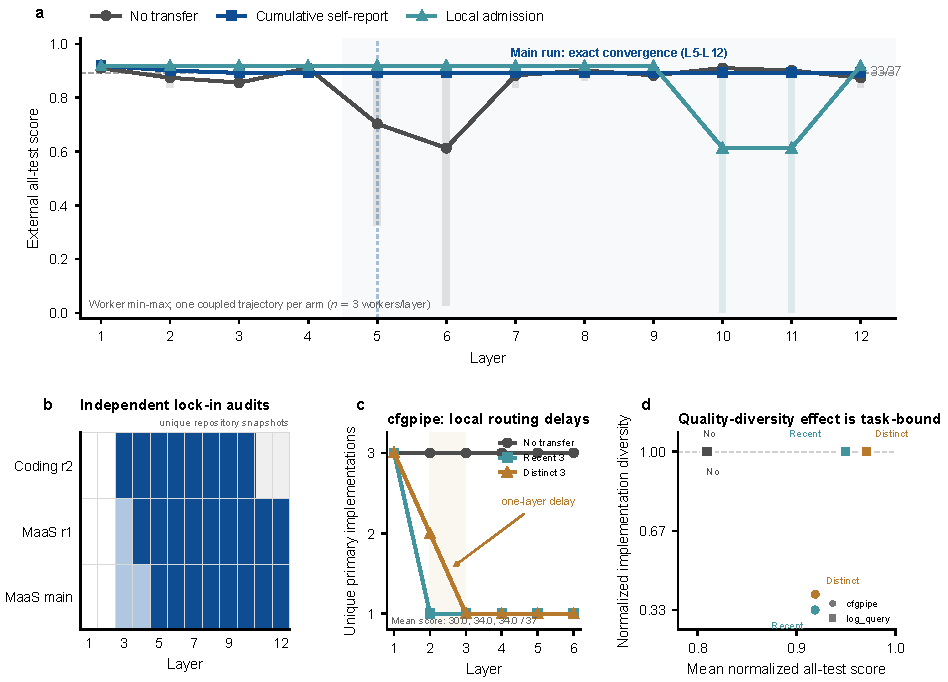
\includegraphics[width=0.90\textwidth]{figures/moa/figure2_depth12_lockin.pdf}
\caption{\textbf{The implementation attractor is reproducible, weakly
mitigated, and task-bound.} \textbf{a}, Frozen main-run external score; ranges
show three-worker minima and maxima. \textbf{b}, Unique full-workspace snapshots
in two retrospective cumulative replications and the frozen main run; dark cells
denote exact three-worker convergence. \textbf{c}, Prospective cfgpipe
primary-implementation diversity. Fixed-recent routing locks at layer 2; the
local-only diversity router retains two implementations at layer 2 but locks from
layer 3, with no quality change. \textbf{d}, Mean normalized score versus
normalized post-layer-1 primary-implementation diversity. Transfer improves score
on both tasks, but reduces diversity only on cfgpipe. Circles denote cfgpipe and
squares denote the prospectively frozen same-provider \texttt{log\_query}
boundary. All panels are descriptive coupled trajectories, not independent
seeds.}
\label{fig:main}
\end{figure*}

\begin{figure*}[t]
\centering
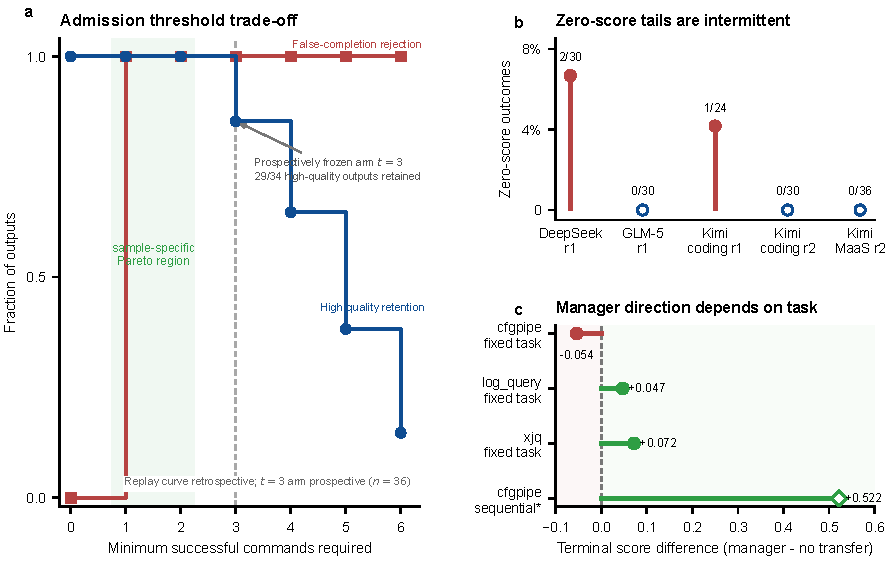
\includegraphics[width=0.93\textwidth]{figures/moa/figure3_admission_boundaries.pdf}
\caption{\textbf{Admission and outcome direction are conditional.}
\textbf{a}, Retrospective threshold replay over all 36 local-arm outputs:
catastrophic rejection is the fraction of two 0/37 outputs rejected, and
high-quality retention is the fraction of 34 outputs scoring at least 33/37 that
are admitted. The replay curve is retrospective, while the marked
three-command arm was prospectively frozen before its outcomes; the shaded
thresholds remain sample-specific rather than validated optima.
\textbf{b}, Valid 0-score event counts under cumulative
self-report across five audited model runs (150 worker outcomes total); rates are
shown separately because layers and providers are not exchangeable.
\textbf{c}, Descriptive terminal treatment-minus-no-transfer score differences
for recursive-manager settings. The sequential \texttt{cfgpipe} control is noisy
and marked with an asterisk; effects are not pooled.}
\label{fig:boundaries}
\end{figure*}

\section{Results}

\subsection{RQ1: Sustained Degradation Is Not Reproduced}

Figure~\ref{fig:main}a shows the frozen 12-layer result. Cumulative self-report
moves from 34/37 at layer 1 to a three-worker mean of 33/37 at layer 3, then
remains exactly at 33/37 through layer 12. It produces no 0/37 events. Thus the
preregistered recurrent catastrophic-tail replication is falsified.

Neither control supports a unique transfer-induced catastrophe. No transfer has
valid action-budget tails of 12/37 and 1/37 at layers 5 and 6, followed by
recovery. Local admission has one 0/37 worker at layer 10 and another at layer
11, so each layer mean falls to 0.613, then all workers return to 34/37 at layer
12. The two local-arm events are independent false-completion trajectories rather
than propagated snapshots: each uses one model step, executes zero commands,
produces no snapshot, and is rejected.

Across raw cumulative self-report runs, DeepSeek-V4-Flash has 2/30 zero-score
events, GLM-5 has 0/30, and Kimi-K2.6 has 1/24 in an initial coding-endpoint run,
0/30 in a preregistered replication, and 0/36 in the fresh MaaS replication
(Figure~\ref{fig:boundaries}b). Every observed valid zero event is isolated or
terminal; none establishes a persistent downward curve. More layers increase the
opportunity to sample rare agent failures, but depth alone is not a sufficient
explanation for sustained degradation.

\subsection{RQ2: Shared Experience Removes Independent Solutions}

The absence of a death spiral does not imply that transfer is inert.
In cumulative self-report, all three workers share one failed-test signature
from layer 3 through layer 12.
At layers 3--4 they occupy two snapshot hashes; from layer 5 onward all 24
remaining outputs are byte-identical directory snapshots. Every layer-3--12
worker passes Core and fails the same four broader tests.

At layer 12, no transfer retains three distinct snapshots, three failed-test
signatures, dominant snapshot share $1/3$, and pairwise failed-test Jaccard
0.278. Both cumulative self-report and local admission end with one snapshot,
one signature, dominant share 1, and Jaccard 1. Local admission therefore blocks
some trajectories but does not preserve terminal implementation diversity among
accepted trajectories.

The same implementation phenomenon recurs outside the main trajectory
(Figure~\ref{fig:main}b). The independent Coding run has three distinct layer-2
snapshots and one shared snapshot from layers 3--10. The independent MaaS run
reaches one snapshot from layers 4--9, experiences an intermittent no-snapshot
0/37 event at layer 10, and reconverges at layer 11. Neither matched no-transfer
control has two consecutive exact-convergence layers.

The prospective bounded arm separates lock-in from cumulative history growth
(Figure~\ref{fig:main}c). Layer 1 contains three distinct 34/37 primary
implementations. From layer 2 through layer 6, all workers produce the same
\texttt{cfgpipe.py} with exactly three references per worker. Full-workspace
hashes differ at layers 4 and 6 only because of an auxiliary \texttt{ws.txt} or
test file; they do not represent primary-implementation re-diversification. At
the first lock-in layers, total input is 1.26--1.60 times the matched no-transfer
load, versus 14.08 times at cumulative layer 12. Accumulating dozens of references
is therefore unnecessary, although transferred context remains a plausible
contributor.

The delivered artifacts contain unusually direct implementation evidence. After
layer 1, 87.9\% of cumulative recipients exactly match at least one prior primary
implementation; their mean maximum source-line Jaccard is 0.965, and 97.6\% of
recipient source lines are available verbatim in at least one delivered snapshot
excerpt. In the bounded arm all three values are 1.0. These measurements support
an implementation-attractor mechanism, while not distinguishing literal copying
from deterministic regeneration conditioned on the same code-rich prompt.

\subsection{RQ3: Local Diversity Routing Delays but Does Not Prevent Lock-In}

The prospective local-only router preserves the three-reference cap but selects
the most recent three distinct implementation identities across all prior layers.
On cfgpipe, bounded-recent diversity AUC over layers 2--6 is 5, the minimum
possible value, and exact primary lock-in begins at layer 2. Diversity-aware
routing raises AUC to 6 by retaining two implementations at layer 2, then locks
from layer 3 through layer 6. Both transfer arms score 34/37 for all 18 outputs,
so this is a one-layer delay without a quality trade-off, not a solution.

The prospectively frozen same-provider \texttt{log\_query} probe is a boundary
rather than a replication (Figure~\ref{fig:main}d). No transfer, bounded recent,
and bounded diverse each retain three primary implementations at every measured
layer. Mean all-test counts are 108.4/134, 127.2/134, and 130.1/134, respectively,
while the two transfer arms both average 9.67/10 Core. Because bounded recent
already reaches the diversity ceiling, no incremental mitigation effect is
identifiable. The cfgpipe attractor is therefore conditional on task and trajectory
rather than an automatic consequence of shared experience.

\subsection{RQ4: Recursive Synthesis Can Privilege a Fixed Point}

The recursive-manager probes show how a compact privileged artifact can stabilize
shared behavior. In the Kimi \texttt{cfgpipe} probe, the manager's layer-3 and
layer-4 playbooks are byte-identical. At layer 5, all recursive workers produce
the same snapshot and score 32/37, whereas no-transfer workers produce three
different snapshots and score 34/37. The manager repeatedly preserves an
incorrect source-precedence rule and two additional edge-case errors. This
supports a fixed-point lock-in mechanism, but the preregistered primary Core
degradation criterion is falsified because both arms retain 4/4 Core.

The DeepSeek stress probe reaches a near-textual manager fixed point. Its three
terminal implementations remain distinct, yet all score 32/37 and fail the same
five tests. Because the score-blinded bootstrap includes an externally failed
source, this is evidence that synthesis compresses mixed-success trajectories
into common behavior, not that locally or globally correct experience becomes
harmful by itself.

The direction does not generalize across tasks
(Figure~\ref{fig:boundaries}c). Recursive synthesis improves terminal normalized
all-test score by 0.047 on \texttt{log\_query} and 0.072 on \texttt{xjq}. A
sequential \texttt{cfgpipe} pilot also favors treatment by 0.522 against a noisy
action-budget control. An \texttt{execution\_server} pilot is descriptively
positive but confirmatorily invalid because no transfer reaches the frozen action
boundary without explicit completion. Shared fixed points can therefore encode
useful stabilization or shared error; task and admission semantics determine the
direction.

\subsection{RQ5: Admission Blocks False Completion at a Cost}

The local gate's three-command threshold was frozen before the 36-output arm was
run. It rejects both observed 0/37 false completions and their artifact identifiers
never occur in later recipient prompts. This is a prospective mechanical
protection against direct propagation in the audited arm.

The same gate rejects seven of 36 outputs: the two 0/37 events and five externally
strong 34/37 outputs that use only two successful commands. We replay thresholds
0--6 on the frozen trajectories (Figure~\ref{fig:boundaries}a). Thresholds 1 or
2 retain all 34 high-quality outputs while rejecting both zero-command events in
this sample; the frozen threshold 3 retains 29/34 high-quality outputs. This is a
retrospective sensitivity result, not evidence that two commands is universally
optimal. It shows that admission quality depends on threshold calibration and that
``more verification'' is not cost-free.

\section{Discussion}

\paragraph{The main risk is loss of optionality.}
Parallel agents are valuable partly because independent trajectories can explore
different implementations and failure modes. In the main run, transfer removes
that optionality long before it creates catastrophic score loss. A system that
reports only mean success may therefore look healthy while all workers share the
same blind spot. Implementation and failed-test diversity are useful companion
metrics for multi-agent coding systems.

\paragraph{Stability and diversity are not monotonic goods.}
The same-provider boundary shows why homogenization cannot be labeled inevitable
or harmful in general. On \texttt{log\_query}, shared experience raises score
without reducing implementation diversity. The engineering objective is not
maximal diversity; it is \emph{validated pluralism}: preserve meaningfully
different candidates until evidence is strong enough to collapse them.

\paragraph{Duplicate suppression is not sufficient mitigation.}
The local diversity router changes one mechanism variable without hidden
evaluation or extra model calls, yet buys only one layer on cfgpipe. Once all
recipients see the same code-rich bundle, distinct sources can still induce the
same preferred implementation. Stronger mitigations may require recipient
heterogeneity, counterfactual task partitions, disagreement-seeking prompts, or
explicit portfolio objectives rather than routing alone.

\paragraph{Admission is a governance problem.}
Self-report admits obvious false completion. A command-count gate catches the
observed zero-command cases but confuses concise work with absent work. Better
admission should combine provenance, task-relevant local tests, change evidence,
uncertainty, and diversity contribution. It should also retain rejected artifacts
for audit rather than silently erasing them.

\paragraph{More layers are not always a better mechanism test.}
Once the shared playbook or snapshots reach a fixed point, additional identical
layers mostly resample stochastic agent execution and inflate context. A stronger
causal test changes one mechanism variable---admission, compression, routing, or
recipient heterogeneity---under a matched control, rather than extending an
already stationary curve.

\section{Limitations}

The strongest confirmatory result remains one frozen Kimi provider run on one
\texttt{cfgpipe} checkpoint with three workers per layer. Two independent
cumulative trajectories reproduce exact lock-in retrospectively, but they were
not preregistered for that metric and do not provide an inferential sampling
distribution. The bounded-context control is one prospective trajectory and does
not equalize every input token. The diversity-router arm reuses already observed
frozen controls, has one trajectory, and tests only exact local identity
deduplication. The same-provider \texttt{log\_query} boundary is prospective but
only three layers deep, so later lock-in remains possible. Neither prospective
probe provides independent seeds, larger worker cohorts, temperature sweeps, or
heterogeneous models. Cross-model audits use different provider endpoints and are
not statistical replications of one immutable model binary.
SlopCodeBench tasks are executable and realistic enough to expose coding behavior,
but they do not cover browser work, long-lived organizations, or asynchronous
agents. The recursive probes differ in admission semantics; the DeepSeek probe has
a mixed-quality bootstrap, and some sequential controls are action-budget noisy or
censored. The gate arm is prospective, but the threshold sweep is retrospective.
Full-workspace equality can overstate implementation change when harmless
auxiliary files differ; we therefore use primary entrypoint hashes for new
prospective endpoints, but historical replications retain full snapshots.
Failed-test equality can still understate latent differences not covered by the
evaluator. We therefore claim a bounded, audited failure mode and trade-off, not
a universal law of multi-agent learning.

\section{Conclusion}

Repeated shared experience did not produce the sustained ant-mill-style degradation
curve we sought. It produced a more defensible result: parallel coding agents can
rapidly lose implementation and behavioral independence, repeatedly enter a
shared implementation attractor, and still maintain apparently strong aggregate
scores. Exact lock-in recurs across three cumulative trajectories and appears
under a fixed-three-reference control, so cumulative history growth is not
necessary in the tested setting. Local identity-aware routing delays lock-in by
one layer but does not prevent it. The prospectively frozen same-provider
\texttt{log\_query} boundary retains maximal implementation diversity while
transfer improves quality, showing that the attractor is task-conditional rather
than universal. Catastrophic tails are intermittent and model-dependent;
recursive synthesis can help or hurt; and local admission blocks false completion
only by choosing a threshold with false-rejection cost. Multi-agent systems should
therefore evaluate not only whether shared experience improves the mean, but also
what diversity it removes, what evidence admits it, and whether mitigation remains
effective beyond the next layer.

\bibliography{antmill}

\end{document}
